\documentclass{standalone}
\usepackage{tikz}
\usetikzlibrary{shapes,snakes}
\begin{document}
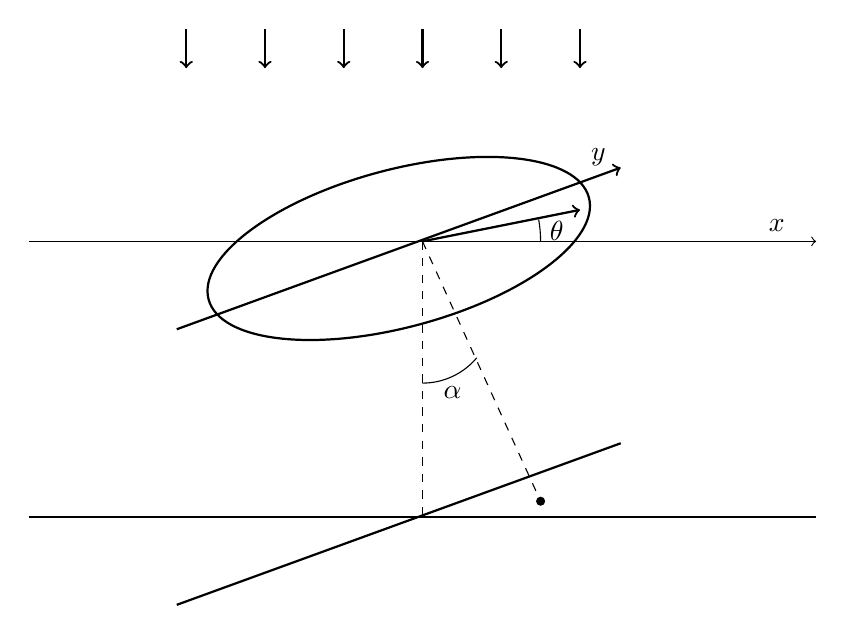
\begin{tikzpicture}
	\draw [->] (0,0.3) -- (10,0.3) node [pos=0.95, above] {$x$};
	\begin{scope}[shift={(0,-1.5)},rotate=20]	
	\draw (5,0) node[ellipse, ,rotate=15, thick, minimum height=2cm,minimum width=5cm,draw] {};
	\draw [->, thick] (2,0) -- (8,0) node [pos=0.95, above] {$y$};
	\end{scope}
	\begin{scope}[shift={(0,-5)},rotate=20]
	\draw [thick] (2,0) -- (8,0) ;
	\end{scope}
	\foreach \x in {2,3,4,5,6,7}
	{
		\draw [thick, ->] (\x,3) -- (\x,2.5);
	}
	\draw [dashed] (5,0.3) -- (5,-3.2);
	\draw [thick]  (0,-3.2) -- (10,-3.2);
	\draw [dashed] (5,0.3) -- (6.5,-3);
	\draw [fill] (6.5,-3) circle (0.05);
	\draw (5,-1.5) arc (90:140:-0.9) node [below, midway] {$\alpha$};
	\draw [thick, ->] (5,0.3) -- (7,0.7);
	\draw (6.5,0.3) arc (0:10:1.6) node [right, midway] {$\theta$};
\end{tikzpicture}
\end{document}